\documentclass{article}
\usepackage[utf8]{inputenc}
\usepackage[margin = 0.8in]{geometry}
\usepackage{graphicx}
\usepackage{amsmath, amssymb}
\usepackage{subcaption}
\usepackage{multirow}
\usepackage{mathtools}
\usepackage{float}


\title{RBE595 - Week 7 Assignment}
\author{Keith Chester}
\date{Due date: February 26, 2023}

\begin{document}
\maketitle

In this assignment, we aimed to create a SARSA and a Q-Learning agent for a 2-dimensional grid world. In this world, there exists terminal states - a goal position, and "cliffs". Falling off of a cliff returns a reward of $-100$, and every transition brings in a reward of $-1$.

Attached to this document in Figure 1 is the SARSA and Q-Learning outcomes with $\alpha=0.1,\epsilon=0.05$ and $10,000$ episodes. Here we see that the SARSA prefers either the middle or top route, whereas Q-Learning chooses the optimal route along the cliff. This is because SARSA utilizes epsilon-greedy action selection when calculating possible next-step rewards, which results in the next-step value occasionally being the large $-100$ reward. This means that the perceived value of cells near the cliffs are lower than what they should be. Q-Learning utilizes a straight Q-max selection which avoids this. Figure 2 presents a plot of the rewards after each episode. This plot shows a general convergence, with epsilon greedy creating occasional spikes of $-100$ rewards to cause the seemingly "wide" drops throughout the chart.

\begin{figure}
    \begin{subfigure}{.5\textwidth}
        \centering
        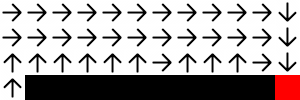
\includegraphics[width=.8\linewidth]{imgs/sarsa.png}
        \caption{SARSA Agent}
    \end{subfigure}
    \begin{subfigure}{.5\textwidth}
        \centering
        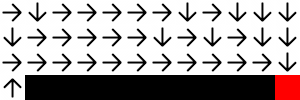
\includegraphics[width=.8\linewidth]{imgs/qlearning.png}
        \caption{Q-Learning Agent}
    \end{subfigure}
    \caption{Agent paths}
\end{figure}

\begin{figure}
    \begin{subfigure}{.5\textwidth}
        \centering
        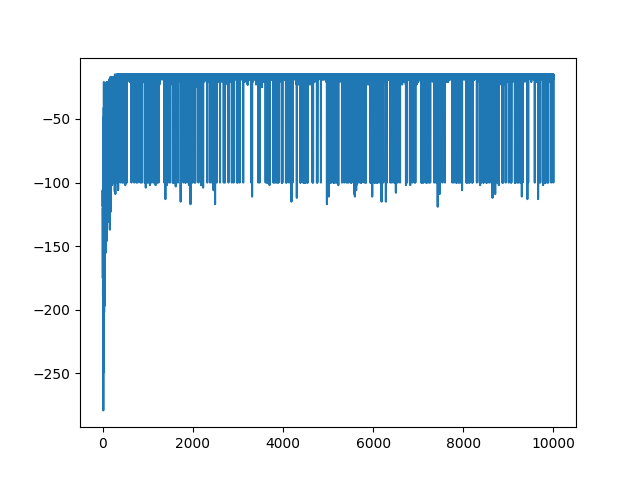
\includegraphics[width=.8\linewidth]{imgs/sarsa_rewards.png}
        \caption{SARSA Agent Rewards}
    \end{subfigure}
    \begin{subfigure}{.5\textwidth}
        \centering
        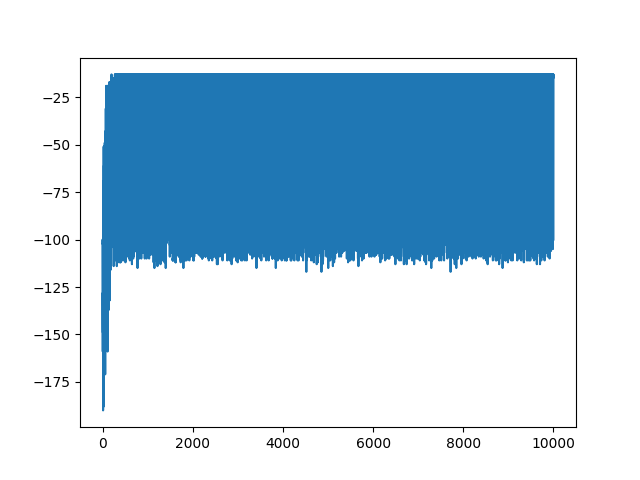
\includegraphics[width=.8\linewidth]{imgs/q_learning_rewards.png}
        \caption{Q-Learning Agent Rewards}
    \end{subfigure}
    \caption{Agent Rewards}
\end{figure}

Why is Q-Learning converging to lower rewards despite finding the optimal route quicker? This is because Q-Learning tends to overestimate the values of future actions, whereas SARSA provides more accurate estimates via taking into account the actual actions taken for the next state. This overestimation leads to a higher probability of Q-Learning choosing suboptimal actions, even though Q-values were high. This is what Doulbe Q-Learning attempts to fix with dual value tracking of Q values for a given state/action pair. Q-Learning finds the optimal route faster as it's off-policy versus the on-policy approach SARSA does.

Finally our Figure 3 demonstrates an experiment where we re-run both models, slowly lowering $\epsilon$ by increments of $0.01$. As $\epsilon$ approaches to $0$ and our exploration moves closer towards a pure $\max Q(S,a)$ approach, SARSA also finds the optimal path instead of staying wary of cliffs.

\begin{figure}
    \begin{subfigure}{.5\textwidth}
        \centering
        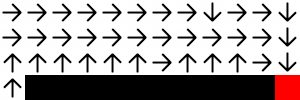
\includegraphics[width=.8\linewidth]{imgs/sarsa_epsilon_0.05.png}
        \caption{SARSA $\epsilon=0.05$}
    \end{subfigure}
    \begin{subfigure}{.5\textwidth}
        \centering
        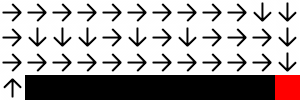
\includegraphics[width=.8\linewidth]{imgs/qlearning_epsilon_0.05.png}
        \caption{Q-Learning $\epsilon=0.05$}
    \end{subfigure}

    \begin{subfigure}{.5\textwidth}
        \centering
        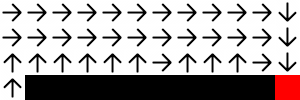
\includegraphics[width=.8\linewidth]{imgs/sarsa_epsilon_0.04.png}
        \caption{SARSA $\epsilon=0.04$}
    \end{subfigure}
    \begin{subfigure}{.5\textwidth}
        \centering
        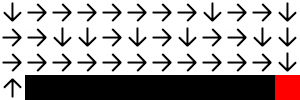
\includegraphics[width=.8\linewidth]{imgs/qlearning_epsilon_0.04.png}
        \caption{Q-Learning $\epsilon=0.04$}
    \end{subfigure}

    \begin{subfigure}{.5\textwidth}
        \centering
        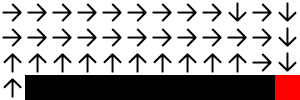
\includegraphics[width=.8\linewidth]{imgs/sarsa_epsilon_0.03.png}
        \caption{SARSA $\epsilon=0.03$}
    \end{subfigure}
    \begin{subfigure}{.5\textwidth}
        \centering
        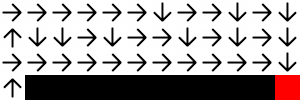
\includegraphics[width=.8\linewidth]{imgs/qlearning_epsilon_0.03.png}
        \caption{Q-Learning $\epsilon=0.03$}
    \end{subfigure}

    \begin{subfigure}{.5\textwidth}
        \centering
        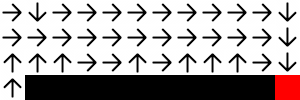
\includegraphics[width=.8\linewidth]{imgs/sarsa_epsilon_0.02.png}
        \caption{SARSA $\epsilon=0.02$}
    \end{subfigure}
    \begin{subfigure}{.5\textwidth}
        \centering
        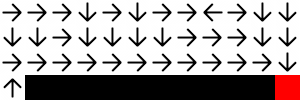
\includegraphics[width=.8\linewidth]{imgs/qlearning_epsilon_0.02.png}
        \caption{Q-Learning $\epsilon=0.02$}
    \end{subfigure}

    \begin{subfigure}{.5\textwidth}
        \centering
        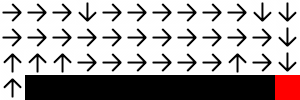
\includegraphics[width=.8\linewidth]{imgs/sarsa_epsilon_0.01.png}
        \caption{SARSA $\epsilon=0.01$}
    \end{subfigure}
    \begin{subfigure}{.5\textwidth}
        \centering
        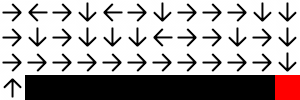
\includegraphics[width=.8\linewidth]{imgs/qlearning_epsilon_0.01.png}
        \caption{Q-Learning $\epsilon=0.01$}
    \end{subfigure}

    \begin{subfigure}{.5\textwidth}
        \centering
        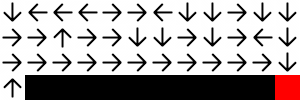
\includegraphics[width=.8\linewidth]{imgs/sarsa_epsilon_0.00.png}
        \caption{SARSA $\epsilon=0.00$}
    \end{subfigure}
    \begin{subfigure}{.5\textwidth}
        \centering
        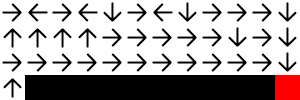
\includegraphics[width=.8\linewidth]{imgs/qlearning_epsilon_0.00.png}
        \caption{Q-Learning $\epsilon=0.00$}
    \end{subfigure}

    \caption{Lowering $epsilon$ by $0.01$ steps}
\end{figure}

\end{document}